% Created 2021-12-10 Fri 21:00
% Intended LaTeX compiler: pdflatex
\documentclass[11pt]{article}
\usepackage[utf8]{inputenc}
\usepackage[T1]{fontenc}
\usepackage{graphicx}
\usepackage{grffile}
\usepackage{longtable}
\usepackage{wrapfig}
\usepackage{rotating}
\usepackage[normalem]{ulem}
\usepackage{amsmath}
\usepackage{textcomp}
\usepackage{amssymb}
\usepackage{capt-of}
\usepackage{hyperref}
\author{Ali Kadum Hassan, Frederik Henriques Altmann, Gustav Emil Mark-Hansen}
\date{\today}
\title{Opg3}
\hypersetup{
 pdfauthor={Ali Kadum Hassan, Frederik Henriques Altmann, Gustav Emil Mark-Hansen},
 pdftitle={Opg3},
 pdfkeywords={},
 pdfsubject={},
 pdfcreator={Emacs 27.2 (Org mode 9.5)}, 
 pdflang={English}}
\begin{document}

\maketitle
\tableofcontents


\section{OPGAVE 1}
\label{sec:orgf48354d}

\subsection{a}
\label{sec:orgb649a2b}
\begin{verbatim}
Hej
\end{verbatim}

\begin{center}
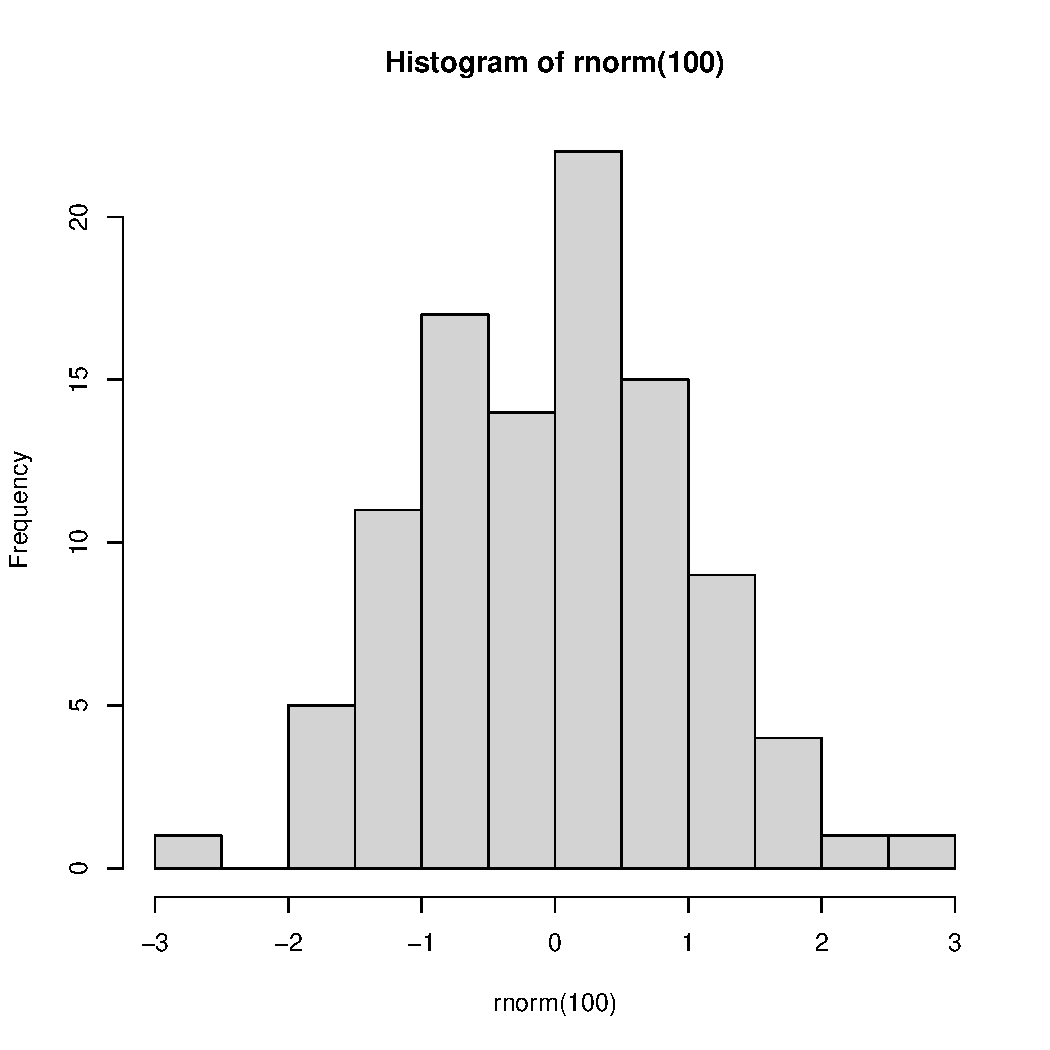
\includegraphics[width=.9\linewidth]{img.png}
\end{center}

Some text
\(e = mc^2\)

\subsection{a}
\label{sec:org40031ec}
Chancen for at få X kast der lander på krone i træk, er:
\((\frac{1}{2})^X\)

Skrevet i R:
\begin{verbatim}
pmf = \(throws) 0.5^throws
\end{verbatim}
\subsection{b}
\label{sec:org9daf217}
Profiten \(f(X)\) er givet ved \(f(a, X) = a2^X - a\)

Skrevet i R:
\begin{verbatim}
profit = \(buyin, throws) buyin * 2^(throws) - buyin
\end{verbatim}
\subsection{c}
\label{sec:org450d4c2}
\begin{align}
E(X) = \sum_{n=1}^\infty |f(b,n)|p(n) = \sum_{n=1}^\infty b \\
|f(x)|p(x) = b2^{x+1}0.5^x = b \\
\sum_{n=1}^\infty |f(b,n)|p(n) = \sum_{n=1}^\infty b = \infty
\end{align}

Da \(E(X)\) divergerer mod positiv uendelig har spillet ikke noget forventet udfald.
\section{2}
\label{sec:org4596370}
\subsection{a}
\label{sec:org97ade03}
Da hele pmf \(p\), bortset fra \(p(x=-1,y=3)\) er kendt kan \(z\) beregnes ved at isolere.

\begin{center}
\begin{tabular}{lrrl}
p(x, y) & y = −1 & y = 1 & y = 3\\
x = −1 & 0.1 & 0.1 & z\\
x = 1 & 0.3 & 0.05 & 0.05\\
\end{tabular}
\end{center}

\begin{align}
\int p(x,y) &= 1 \\
1 &= 0.1 + 0.1 + 0.3 + 0.05 + 0.05 + z = 0.6 + z \\
z &= 1 - 0.6 = 0.4
\end{align}

Skrevet i R:
\begin{verbatim}
p <- matrix(c(0.1,0.1,z,0.3,0.05,0.05), 2, 3, TRUE)
z <- 1 - (0.1 + 0.1 + 0.3 + 0.05 + 0.05)
\end{verbatim}
\subsection{b}
\label{sec:org36a9c81}
Beregn den forventede gevinst

\begin{align}
E[X+Y] &= E[X] + E[Y] \\
E[X] &= -1*0.6 + 1*0.4 = -0.2 \\
E[Y] &= -1*0.4 + 1*0.15 + 3*0.45 = 1.1 \\
E[X+Y] &= 1.1 - 0.2 = 0.9
\end{align}

Skrevet i R (fortsat):

\begin{verbatim}
x <- -sum(p[1,]) + sum(p[2,])
y <- -sum(p[,1]) + sum(p[,2]) + 3*sum(p[,3])
E <- x + y # Forventede gevinst
\end{verbatim}
\subsection{c}
\label{sec:orge7be5fe}
beregn kovariansen mellem X og Y. Er X og Y uafhængige?

Skrevet i R (fortsat):
\begin{verbatim}
xy <- c(z, 0.3+0.1, 0.15, 0.05)
-3*xy[1]+ (-1)*xy[2] +xy[3]+3*xy[4] #-> E(xy) = -1.3
-1.3-(mean(x)*mean(y)) #->              Cov(x,y)= -1.08
\end{verbatim}

Hvilket betyder at de er afhængige af hinanden, da cov /= 0 og at de 2 bevæger sig modsat af hinanden

\section{3}
\label{sec:org68ff1a6}
\subsection{a}
\label{sec:org2c4f44c}
Vi ved at hvis \(A\) har et udfald som er givet,
har den altid en sandsynlighed \(1\) betinget at det er udfaldet.

\begin{center}
\begin{tabular}{lrr}
CPT & A=1 & A=0\\
P(T=1 givet A) & 0.998 & a\\
P(T=0 givet A) & b & 0.993\\
sum & 1 & 1\\
\end{tabular}
\end{center}

Derfor må \(a = 1-0.993\) og \(b=1-0.998\).

\begin{center}
\begin{tabular}{lrr}
CPT & A=1 & A=0\\
P(T=1 givet A) & 0.998 & 0.007\\
P(T=0 givet A) & 0.002 & 0.993\\
sum & 1 & 1\\
\end{tabular}
\end{center}

Sandsynligheden for at have en peanut allergi er \(P(A = 1) = 0.01\), 1\%,
samt \(P(A = 0) = 0.99\), 99\% for ikke at have allergien.

Da
\[P(A|B) = \frac{P(A \union B)}{P(B)}\]
\[P(A \union B) = P(A|B)\cdot P(B)\]

kan en \textbf{pmf} beregnes.

\begin{center}
\begin{tabular}{lrrr}
PMF & A=1 & A=0 & sum\\
T=1 & 0.00998 & 0.00693 & 0.01691\\
T=0 & 0.00002 & 0.98307 & 0.98309\\
sum & 0.01 & 0.99 & 1\\
\end{tabular}
\end{center}

Summen af rækkerne er så hhv. \(P(T=1)\) og \(P(T=0)\).
\subsection{b}
\label{sec:orge5eaf04}
Sandsynligheden for ikke at have allergien givet en negativ test er:
\[P(A=0|T=0)=\frac{P(A=0,T=0)}{P(T=0)}=\frac{0.98307}{0.98309}= 0.9999797\]
\subsection{c}
\label{sec:orgf601823}
Sandsynligheden for at have allergien givet en positiv test er:
\[P(A=1|T=1)=\frac{P(A=1,T=1)}{P(T=1)}=\frac{0.00998}{0.01}= 0.998\]


\section{4}
\label{sec:org06aa44c}
\subsection{a}
\label{sec:org7ec5895}
\end{document}
